\chapter{Sprint 2}

\section{Sprint Goal}
L'obiettivo dello sprint 2 è quello di effettuare l'analisi dei requisiti a partire dall'intervista effettuata precedentemente con l'esperto del dominio, ideare il design generale architetturale e realizzare una prima versione dei mockup da sottoporre poi al committente per avere un riscontro da tenere in considerazione per eventuali modifiche.


\section{Sprint Backlog}
%descrizione del refinement e immagine sprint backlog
Lo sprint backlog risultante:
\begin{figure}[H]
    \centering
    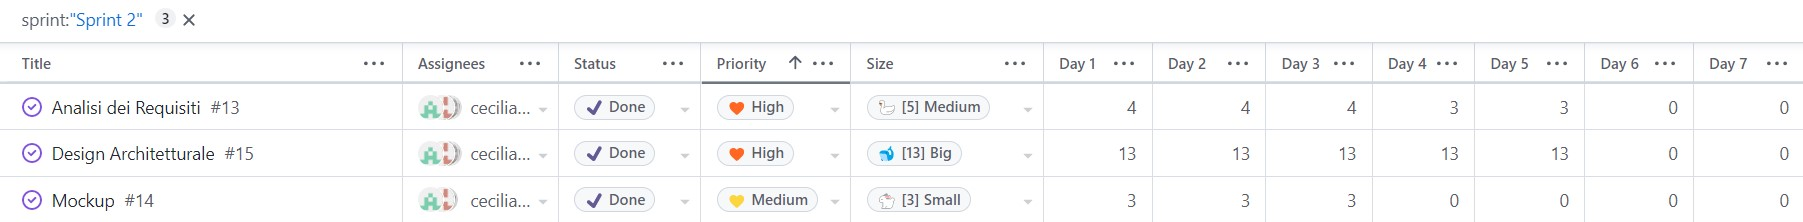
\includegraphics[width=\textwidth]{process/Img/Sprint2BL.jpg}
    \caption{Sprint 2 backlog}
    \label{fig:Sprint2}
\end{figure}

\section{Sprint Review}
%only this part is present also in the main report
%<*partPresentAlsoInReport>
Durante questo sprint abbiamo realizzato l'analisi dei requisiti del sistema e ideata l'architettura generale del sistema, dalla quale sono sorti alcuni dubbi che sono stati poi discussi e chiariti con l'esperto del dominio. Sono state realizzare due versioni dei mockup dell'applicazione, le quali hanno ricevuto entrambe giudizi positivi, ma andranno successivamente unite e raffinate per soddisfare al meglio i requisiti del committente.
\paragraph{Deliverables} 
I deliverables per questo sprint sono stati i seguenti:
\begin{itemize}
    \item Mockup
    \item Diagramma dei casi d'uso
    \item Diagramma delle classi
\end{itemize}
%</partPresentAlsoInReport>


\section{Sprint Retrospective}
Durante il secondo sprint ci sono stati diversi momenti in cui il team si è trovato a dover riflettere su alcuni aspetti che risultavano poco chiari o che non erano stati adeguatamente approfonditi durante l'intervista con l'esperto del dominio. Questo è avvenuto soprattutto durante l'analisi dei requisiti e il design generale dell'architettura. A seguito del confronto eseguito durante uno dei meeting, è stato ritenuto che tali aspetti sono stati chiariti.